%%%%%%%%%%%%%%%%%%%%%%%%%%%%%%%%%%%%%%%%%
% Programming/Coding Assignment
% LaTeX Template
%
% This template has been downloaded from:
% http://www.latextemplates.com
%
% Original author:
% Ted Pavlic (http://www.tedpavlic.com)
%
% Note:
% The \lipsum[#] commands throughout this template generate dummy text
% to fill the template out. These commands should all be removed when 
% writing assignment content.
%
% This template uses a Perl script as an example snippet of code, most other
% languages are also usable. Configure them in the "CODE INCLUSION 
% CONFIGURATION" section.
%
%%%%%%%%%%%%%%%%%%%%%%%%%%%%%%%%%%%%%%%%%

%----------------------------------------------------------------------------------------
%	PACKAGES AND OTHER DOCUMENT CONFIGURATIONS
%----------------------------------------------------------------------------------------

\documentclass{article}

\usepackage{fancyhdr} % Required for custom headers
\usepackage{lastpage} % Required to determine the last page for the footer
\usepackage{extramarks} % Required for headers and footers
\usepackage[usenames,dvipsnames]{color} % Required for custom colors
\usepackage{graphicx} % Required to insert images
\usepackage{subcaption}
\usepackage{listings} % Required for insertion of code
\usepackage{courier} % Required for the courier font
\usepackage{lipsum} % Used for inserting dummy 'Lorem ipsum' text into the template
\usepackage{enumerate}
\usepackage{amssymb}
\usepackage{amsmath}
\usepackage{array}
\usepackage{forloop}
\usepackage{alphalph}
\renewcommand*{\thesubfigure}{%
\alphalph{\value{subfigure}}%
}%
% !TeX spellcheck = en_GB

% Margins
\topmargin=-0.45in
\evensidemargin=0in
\oddsidemargin=0in
\textwidth=6.5in
\textheight=9.0in
\headsep=0.25in

\linespread{1.1} % Line spacing

% Set up the header and footer
\pagestyle{fancy}
\lhead{\hmwkAuthorName} % Top left header
\chead{\hmwkClass\ (\hmwkClassTime): \hmwkTitle} % Top center head
%\rhead{\firstxmark} % Top right header
\lfoot{\lastxmark} % Bottom left footer
\cfoot{} % Bottom center footer
\rfoot{Page\ \thepage\ of\ \protect\pageref{LastPage}} % Bottom right footer
\renewcommand\headrulewidth{0.4pt} % Size of the header rule
\renewcommand\footrulewidth{0.4pt} % Size of the footer rule

\setlength\parindent{0pt} % Removes all indentation from paragraphs

%----------------------------------------------------------------------------------------
%	CODE INCLUSION CONFIGURATION
%----------------------------------------------------------------------------------------

\definecolor{MyDarkGreen}{rgb}{0.0,0.4,0.0} % This is the color used for comments
\lstset{language=Python,
        frame=single, % Single frame around code
        basicstyle=\small\ttfamily, % Use small true type font
        keywordstyle=[1]\color{Blue}\bf,
        keywordstyle=[2]\color{Purple},
        keywordstyle=[3]\color{Blue}\underbar,                            
        commentstyle=\usefont{T1}{pcr}{m}{sl}\color{MyDarkGreen}\small,
        stringstyle=\color{Purple},
        showstringspaces=false,
        tabsize=5,
        %
        % Put standard functions not included in the default language here
        morekeywords={rand},
        %
        % Put function parameters here
        morekeywords=[2]{on, off, interp},
       	%
        morecomment=[l][\color{Blue}]{...},
        numbers=left, % Line numbers on left
        firstnumber=1, % Line numbers start with line 1
        numberstyle=\tiny\color{Blue}, % Line numbers are blue and small
        stepnumber=1
}

%----------------------------------------------------------------------------------------
%	DOCUMENT STRUCTURE COMMANDS
%	Skip this unless you know what you're doing
%----------------------------------------------------------------------------------------

% Header and footer for when a page split occurs within a problem environment
\newcommand{\enterProblemHeader}[1]{
%\nobreak\extramarks{#1}{#1 continued on next page\ldots}\nobreak
%\nobreak\extramarks{#1 (continued)}{#1 continued on next page\ldots}\nobreak
}

% Header and footer for when a page split occurs between problem environments
\newcommand{\exitProblemHeader}[1]{
%\nobreak\extramarks{#1 (continued)}{#1 continued on next page\ldots}\nobreak
%\nobreak\extramarks{#1}{}\nobreak
}

\setcounter{secnumdepth}{0} % Removes default section numbers
\newcounter{homeworkProblemCounter} % Creates a counter to keep track of the number of problems
\setcounter{homeworkProblemCounter}{0}

\newcommand{\homeworkProblemName}{}
\newenvironment{homeworkProblem}[1][Part \arabic{homeworkProblemCounter}]{ % Makes a new environment called homeworkProblem which takes 1 argument (custom name) but the default is "Problem #"
\stepcounter{homeworkProblemCounter} % Increase counter for number of problems
\renewcommand{\homeworkProblemName}{#1} % Assign \homeworkProblemName the name of the problem
\section{\homeworkProblemName} % Make a section in the document with the custom problem count
\enterProblemHeader{\homeworkProblemName} % Header and footer within the environment
}{
\exitProblemHeader{\homeworkProblemName} % Header and footer after the environment
}

\newcommand{\problemAnswer}[1]{ % Defines the problem answer command with the content as the only argument
\noindent\framebox[\columnwidth][c]{\begin{minipage}{0.98\columnwidth}#1\end{minipage}} % Makes the box around the problem answer and puts the content inside
}

\newcommand{\homeworkSectionName}{}
\newenvironment{homeworkSection}[1]{ % New environment for sections within homework problems, takes 1 argument - the name of the section
\renewcommand{\homeworkSectionName}{#1} % Assign \homeworkSectionName to the name of the section from the environment argument
\subsection{\homeworkSectionName} % Make a subsection with the custom name of the subsection
\enterProblemHeader{\homeworkProblemName\ [\homeworkSectionName]} % Header and footer within the environment
}{
\enterProblemHeader{\homeworkProblemName} % Header and footer after the environment
}
\setlength\parindent{0pt}
%----------------------------------------------------------------------------------------
%	NAME AND CLASS SECTION
%----------------------------------------------------------------------------------------

\newcommand{\hmwkTitle}{Project\ \#2} % Assignment title
\newcommand{\hmwkDueDate}{Sunday,\ February\ 23,\ 2018} % Due date
\newcommand{\hmwkClass}{CSC411} % Course/class
\newcommand{\hmwkClassTime}{L0101} % Class/lecture time
\newcommand{\hmwkAuthorName}{Hao Zhang \& Tyler Gamvrelis} % Your name

%----------------------------------------------------------------------------------------
%	TITLE PAGE
%----------------------------------------------------------------------------------------

\title{
\vspace{2in}
\textmd{\textbf{\hmwkClass:\ \hmwkTitle}}\\
\normalsize\vspace{0.1in}\small{Due\ on\ \hmwkDueDate}\\
\vspace{0.1in}
\vspace{3in}
}

\author{\textbf{\hmwkAuthorName}}
%\date{} % Insert date here if you want it to appear below your name

%----------------------------------------------------------------------------------------

\begin{document}

\maketitle
\clearpage
%----------------------------------------------------------------------------------------
%	PROBLEM 1
%-------------------------------------------------------------------------------------
\clearpage
\section{Foreword}
In this project, neural networks of various depth were used to recognize handwritten digits and faces.
\newline
\newline
Part 1 provides a description of the MNIST dataset from which the images of handwritten digits were taken. Part 2 implements the computation of a simple network. Part 3 presents the \textit{sum of the negative log-probabilities} as a cost function, and derives the expression for its gradient with respect to one of its weights. Part 4 details the training and optimization procedures for a digit-recognition neural network, and part 5 improves upon the results by modifying gradient descent to use momentum. Learning curves are presents in parts 4 and 5. Part 6 presents an analysis of network behaviour with respect to two of its weights. Part 7 provides an analysis of the performance of two different backpropagation computation techniques. Part 8 presents a face recognition network architecture for classifying actors, and uses PyTorch for implementation. Part 9 presents visualizations of hidden unit weights relevant to two of the actors. Part 10 uses activations of AlexNet to train a neural network to perform classification of the actors.
\newline
\newline
\textbf{System Details for Reproducibility:}
\begin{itemize}
	\item Python 2.7.14
	\item Libraries:
	\begin{itemize}
		\item numpy
		\item matplotlib
		\item pylab
		\item time
		\item os
		\item scipy
		\item urllib
		\item cPickle
		\item PyTorch
	\end{itemize}
\end{itemize}
\clearpage


% Part 1
\begin{homeworkProblem}
\noindent \textit{Dataset description}

\noindent The MNIST dataset is made of thousands of 28 by 28 pixel images of the handwritten digits: 0 to 9. The images are split into training set and test set images labelled `train0' to `train9' and `test0' to `test9'. The number of images with each label is presented in Table~\ref{tab:part1_MNIST}, below.

\begin{table}[!ht]
\begin{center}
\begin{tabular}{ | m{3em} | m{4cm}| m{3em} | m{4cm}| } 
\hline
\textbf{Label} & \textbf{Number of Images}  &\textbf{Label} & \textbf{Number of Images}\\ 
\hline
train0 & 5923  &test0 & 980\\ 
\hline
train1 & 6742  &test1 & 1135\\ 
\hline
train2 & 5958  &test2 & 1032\\ 
\hline
train3 & 6131  &test3 & 1010\\ 
\hline
train4 & 5842  &test4 & 982\\ 
\hline
train5 & 5421  &test5 & 892\\ 
\hline
train6 & 5918  &test6 & 958\\ 
\hline
train7 & 6265  &test7 & 1028\\ 
\hline
train8 & 5851  &test8 & 974\\ 
\hline
train9 & 5949  &test9 & 1009\\ 
\hline
\end{tabular}
\end{center}
\caption{Quantity of each type of image in the MNIST dataset.}
\label{tab:part1_MNIST}
\end{table}

Ten images of each number were taken from the training sets and displayed in Figure~\ref{fig:numberExamples}. The correct labels of most of the pictures can be discerned at a glance by humans However, since the digits are handwritten, some of them may not be completely obvious. For example, Figure~\ref{fig:example99} is categorized as a 9 but looks like an 8.

\newcounter{ith}
\newcounter{num}
\begin{figure*}[ht!]
\centering


\forloop{num}{0}{\value{num} < 10}{
	\forloop{ith}{0}{\value{ith} < 10}{
	\begin{subfigure}{0.08\textwidth}
    	\centering
    	\includegraphics[scale=1, width=1\linewidth]{images/number\arabic{num}_\arabic{ith}.jpg}
    	\caption{}
    	\label{fig:example\arabic{num}\arabic{ith}}
	\end{subfigure}
	}
}


\caption{Subset of the MNIST dataset.}
\label{fig:numberExamples}
\end{figure*}
\clearpage
\end{homeworkProblem}


% Part 2
\begin{homeworkProblem}
\noindent \textit{Computing a Simple Network}

\noindent In this part, the simple network depicted in Figure~\ref{fig:part2_simple_network} was implemented as a function in Python using NumPy, the code listing for which is presented is Figure~\ref{fig:part2_code}.

\begin{figure}[!ht]
	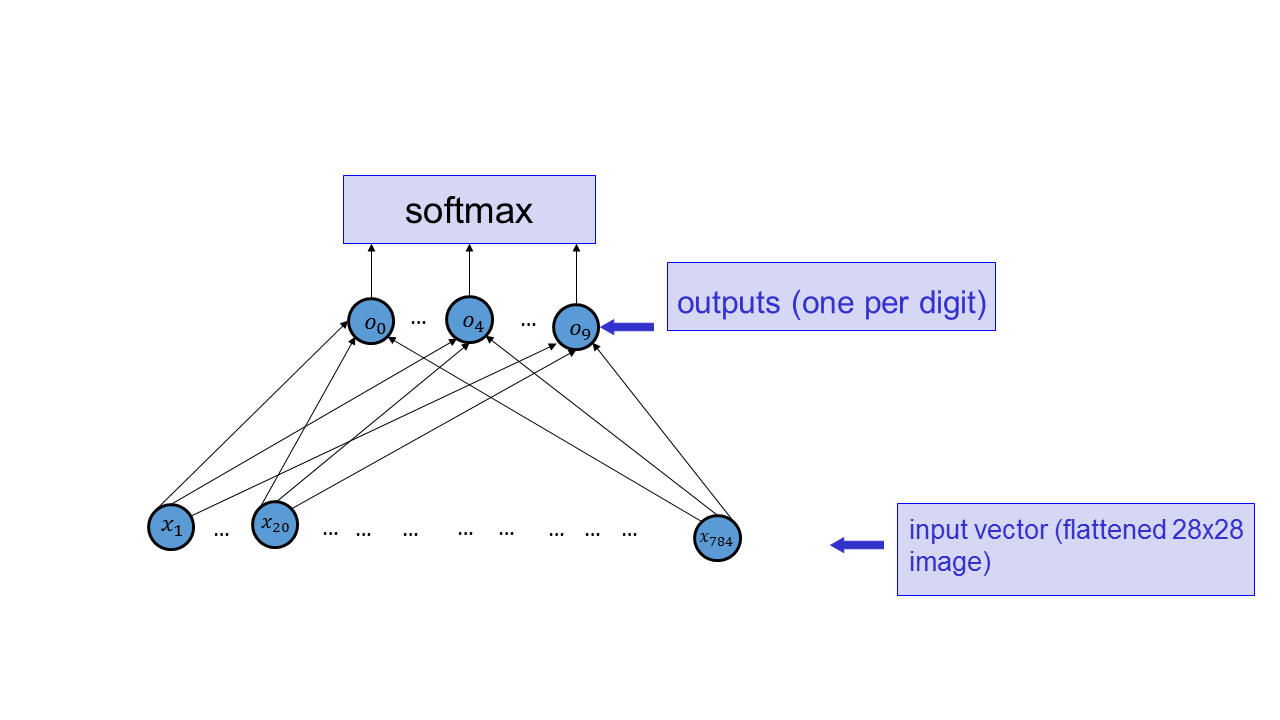
\includegraphics[scale=1, width=1\linewidth]{images/part2_simple_network}
	\caption{Simple network diagram from project handout.}
	\label{fig:part2_simple_network}
\end{figure}

\begin{figure}[!ht]
	\begin{lstlisting}
def softmax(y):
	'''
	Return the output of the softmax function for the matrix of output y. y
	is an NxM matrix where N is the number of outputs for a single case, and M
	is the number of cases
	'''
	return exp(y)/tile(sum(exp(y),0), (len(y),1))

def SimpleNetwork(W, X):
    '''
	SimpleNetwork returns the vectorized multiplication of the (n x 10) 
	parameter matrix W with the data X.
	Arguments:
		W -- (n x 10) matrix of parameters (weights and biases)
		x -- (n x m) matrix whose i-th column corresponds to the i-th training 
	image
	'''
	return softmax(np.dot(W.T, X))
	\end{lstlisting}
	\caption{Python implementation of network using NumPy.}
	\label{fig:part2_code}
\end{figure}

\clearpage
\end{homeworkProblem}


% Part 3
\begin{homeworkProblem}
	\noindent \textit{Cost Function of Negative Log Probabilities}
	
	The Cost function that will be used for the network described in part 2 is:
	$$C = - \sum_{q = 1}^{m} (\sum_{l = 1}^{k} y_llog(p_l))_q$$
	Where $k$ is the number of output nodes, $m$ is the number of training samples, $p_l = \frac{e^{o_l}}{\sum_{c = 1}^{k} e^{o_c}}$ and $y_l$ is equal to $1$ if the training sample is labelled as $l$ and 0 otherwise.\newline
	\break
	
	\noindent \textit{Partial Derivative of the Cost Function (3a)}
	
	Let the matrix $W =  \begin{bmatrix}
    w_{11}       &w_{12} & w_{13} & \dots & w_{1k} \\
    w_{21}       &w_{22} & w_{23} & \dots & w_{2k} \\
    \hdotsfor{5} \\
    w_{n1}       &w_{n2} & w_{n3} & \dots & w_{nk}
\end{bmatrix}$ and let $W_j$ be the $j^{th}$ column of matrix $W$. This results in $o_j = W_j^Tx$ where
$x = \begin{bmatrix}
    x_{1} \\
    x_{2} \\
    \hdotsfor{1} \\
    x_{n} 
\end{bmatrix}$ and $n$ is equal to the number of pixels with an extra $1$ to multiply into the bias. That is, $x_1 ^q$ is always taken to be $1$ while $x_2 ^q,...,x_n ^q$ are the inputs to the network corresponding to the $q^{th}$ training example. \newline

	To calculate the partial derivative of C, we will consider only \textbf{a single training sample}: 
	$C = - \sum_{l = 1}^{k} y_llog(p_l)$
	By the chain rule, the partial derivative with respect to $w_{ij}$ is:
	$$\frac{\partial C(W)}{\partial w_{ij}} = - \sum_{l = 1}^{k} \frac{\partial C}{\partial p_l}\frac{\partial p_l}{\partial o_j}\frac{\partial o_j}{\partial w_{ij}}$$
	The first term is straight forward: $\frac{\partial C}{\partial p_l} = \frac{y_l}{p_l}$.\newline
	
	For the second term, we have $\frac{\partial p_l}{\partial o_j} = 
	\begin{cases}\frac{-e^{o_l}e^{o_j}}{(\sum_{c = 1}^{k} e^{o_c})^2} = -p_lp_j, \text{if } l \ne j\\
	\frac{e^{o_j}}{\sum_{c = 1}^{k} e^{o_c}} - \frac{e^{2o_j}}{(\sum_{c = 1}^{k} e^{o_c})^2} = p_j - p_j^2, \text{if } l = j
	 \end{cases}$

	
	From the equation: $o_j = W_j^Tx$, we have $o_j = w_{1j}x_1 + w_{2j}x_2 + \dots + w_{nj}x_n$ and it is clear to see that: $\frac{\partial o_j}{\partial w_{ij}} = x_i$.\newline
	
	Putting it all together, we have:
	$$\frac{\partial C(W)}{\partial w_{ij}} = - (\sum_{l \ne j} (-\frac{y_l}{p_l}p_lp_j) + \frac{y_j}{p_j}(p_j - p_j^2))x_i = (\sum_{l \ne j} (y_lp_j) + y_j(p_j - 1))x_i$$
	Considering that we are using 1-hot encoding, only a single $y_l$ can equal 1. Therefore, $$\frac{\partial C(W)}{\partial w_{ij}} = \begin{cases}
    (p_j - 1)x_i,& \text{if } y_j = 1\\
    p_jx_i,              & \text{otherwise}
\end{cases}$$
Which is equivalent to saying: $\frac{\partial C(W)}{\partial w_{ij}} = (p_j - y_j)x_i$. To extend this to all training samples, we just have to sum up each individual contribution, resulting in the equation: $\frac{\partial C(W)}{\partial w_{ij}} = \sum_{q = 1}^{m}((p_j - y_j)x_i)_q$.
\clearpage

\noindent \textit{Vectorized Implementation of Gradient (3b)}

To vectorize the gradient, we first define the gradient matrix to be:  $$\frac{\partial C(W)}{\partial W} = 
\begin{bmatrix}
    \frac{\partial C}{w_{11}}       &\dots & \dots & \dots & \frac{\partial C}{w_{1k}} \\
    \frac{\partial C}{w_{21}}       &\dots & \dots & \dots & \frac{\partial C}{w_{2k}} \\
    \hdotsfor{5} \\
    \frac{\partial C}{w_{n1}}       &\dots & \dots & \dots & \frac{\partial C}{w_{nk}}
\end{bmatrix} = \begin{bmatrix}
    \sum_{q = 1}^{m}((p_1 - y_1)x_1)_q       &\dots & \dots & \dots & \sum_{q = 1}^{m}((p_k - y_k)x_1)_q \\
    \sum_{q = 1}^{m}((p_1 - y_1)x_2)_q       &\dots & \dots & \dots & \sum_{q = 1}^{m}((p_k - y_k)x_2)_q \\
    \hdotsfor{5} \\
    \sum_{q = 1}^{m}((p_1 - y_1)x_n)_q       &\dots & \dots & \dots & \sum_{q = 1}^{m}((p_k - y_k)x_n)_q
\end{bmatrix}$$

This is equivalent to: $ X(P - Y)^T$ where: $$X = \begin{bmatrix}
    x_{1}^{(1)}       & x_{1}^{(2)} & x_{1}^{(3)} & \dots & x_{1}^{(m)} \\
    x_{2}^{(1)}       & x_{2}^{(2)} & x_{2}^{(3)} & \dots & x_{2}^{(m)} \\
    \hdotsfor{5} \\
    x_{n}^{(1)}       & x_{n}^{(2)} & x_{n}^{(3)} & \dots & x_{n}^{(m)}
\end{bmatrix}
Y = \begin{bmatrix}
    y_{1}^{(1)}       & y_{1}^{(2)} & y_{1}^{(3)} & \dots & y_{1}^{(m)} \\
    y_{2}^{(1)}       & y_{2}^{(2)} & y_{2}^{(3)} & \dots & y_{2}^{(m)} \\
    \hdotsfor{5} \\
    y_{k}^{(1)}       & y_{k}^{(2)} & y_{k}^{(3)} & \dots & y_{k}^{(m)}
\end{bmatrix}
P =  \begin{bmatrix}
    p_{1}^{(1)}       & p_{1}^{(2)} & p_{1}^{(3)} & \dots & p_{1}^{(m)} \\
    p_{2}^{(1)}       & p_{2}^{(2)} & p_{2}^{(3)} & \dots & p_{2}^{(m)} \\
    \hdotsfor{5} \\
    p_{k}^{(1)}       & p_{k}^{(2)} & p_{k}^{(3)} & \dots & p_{k}^{(m)}
\end{bmatrix}$$
Where the superscript of each element represents the index of the training samples. The code used to compute the gradient is shown in Figure~\ref{fig:part3_gradient}.
\newline
\begin{figure}[!ht]
	\begin{lstlisting}
def negLogLossGrad(X, Y, W):
    '''
    negLogLossGrad returns the gradient of the cost function of negative log
    probabilities.
    
    Arguments:
        X -- Input image(s) from which predictions will be made (n x m)
        Y -- Target output(s) (actual labels) (10 x m)
        W -- Weight matrix (n x 10)
    '''
    
    P = SimpleNetwork(W, X) # Get the prediction for X using the weights W

    return np.dot(X, (P - Y).transpose())
	\end{lstlisting}
	\caption{Vectorized Implementation of the Negative Log Loss Gradient}
	\label{fig:part3_gradient}
\end{figure}
\clearpage


\noindent \textit{Finite Difference Approximation (3b)}
\newline
To check that the gradient was computed correctly, the gradient with respect to weight $w_{ij}$ was approximated using finite differences, for all coordinates in the weight matrix. $10$ values for the differential quantity, $h$, were tested, for which the maximum total error was $2.698$ for $h = 1$ and the minimum total error was $3.054 \times 10^{-7}$ for $h = 1 \times 10^{-7}$. Thus, for sufficiently small $h$, the finite difference approximation and vectorized computation converge to the same quantity, suggesting the vectorized computation is correct. The test case used to obtain this result is shown in Figure~\ref{fig:part3_test}. The complete results are summarized in Table~\ref{tab:part3_grad}, below.
\begin{table}[!ht]
\begin{center}
\begin{tabular}{ | m{12em} | m{2cm} | }
\hline
\textbf{Total error} & \textbf{h}\\
\hline
2.698202291518717  &1.0\\
\hline
0.200166359876926  &0.1\\
\hline
0.019912135073950066  &0.01\\
\hline
0.0019906216532900034  &0.001\\
\hline
0.00019905646908402463  &0.0001\\
\hline
1.990372311189148e-05  &1e-05\\
\hline
1.9841905873896337e-06  &1e-06\\
\hline
3.2450363651737035e-07  &1e-07\\
\hline
3.0542104362263345e-06  &1e-08\\
\hline
2.747131061797692e-05  &1e-09\\
\hline
\end{tabular}
\end{center}
\caption{Sum of differences between vectorized gradient computation and finite difference approximation for $10$ $h$-values.}
\label{tab:part3_grad}
\end{table}


\begin{figure}[!ht]
	\begin{lstlisting}    
# Test part 3
X = [[1, 2, 3, 4], [1, 2, 3, 4], [1, 2, 3, 4], [1, 2, 3 ,4],[1, 2, 3, 4]]
X = np.array(X)
W = [[1, 0, 1.2, 3], [1, 2, 0.2, 1.2], [1, 8, 1, 4], [1, -2, 3, 1], [1, 0, 3, 1]]
W = np.array(W)
Y = [[1, 0, 0, 0], [0, 1, 0, 0], [0, 0, 1, 0], [0, 0, 0, 1]]
Y = np.array(Y)
G1 = negLogLossGrad(X, Y, W)
h = 1.0
for i in range(10):
    G2 = negLogLossGrad_FiniteDifference(X, Y, W, h)
    print "Total error: ", sum(abs(G1 - G2)), "h: ", h
    h /= 10
	\end{lstlisting}
	\caption{Test Case Used to Calculate Error Between Finite Difference Approximation and the Vectorized Gradient}
	\label{fig:part3_test}
\end{figure}
\clearpage
\end{homeworkProblem}


% Part 4
\begin{homeworkProblem}
In this section, the neural network from part 2 was trained using vanilla gradient descent. The optimization procedure is described below, and learning curves and visualizations of the weights going into each of the output units are presented.
\newline
\newline
\noindent \textit{Optimization Procedure}
\newline
%State how we initialized weights and what learning rate we used
Words
\newline
\newline
\noindent \textit{Learning Curves}
\newline
	\begin{figure}[!ht]
	\begin{subfigure}[b]{0.5\textwidth}
    	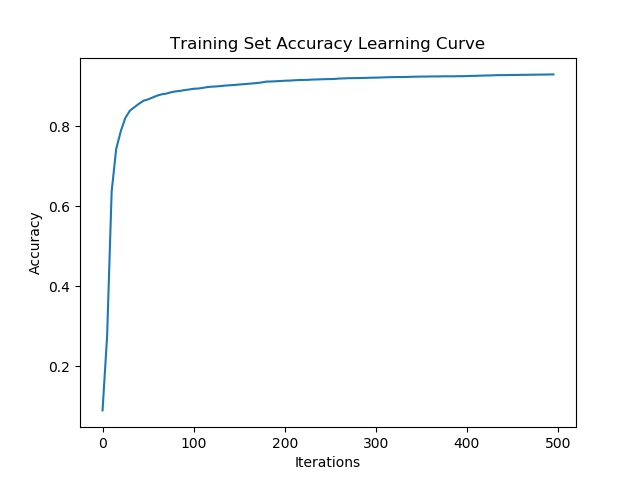
\includegraphics[width=\textwidth]{images/p4_training_set_acc.jpeg}
    	\caption{Performance Curve on the Training Set}
		\label{fig:part4trainPerf}
	\end{subfigure}
%
	\begin{subfigure}[b]{0.5\textwidth}
		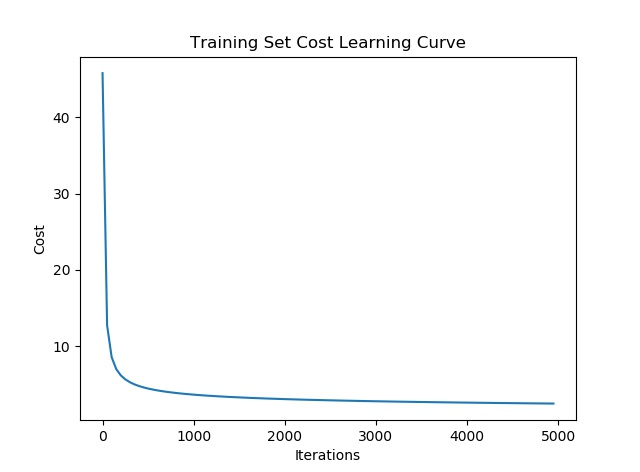
\includegraphics[width=\textwidth]{images/p4_training_set_cost.jpeg}
		\caption{Loss Curve on the Training Set}
		\label{fig:part4trainLoss}
	\end{subfigure}
    %	
	\begin{subfigure}[b]{0.5\textwidth}
    	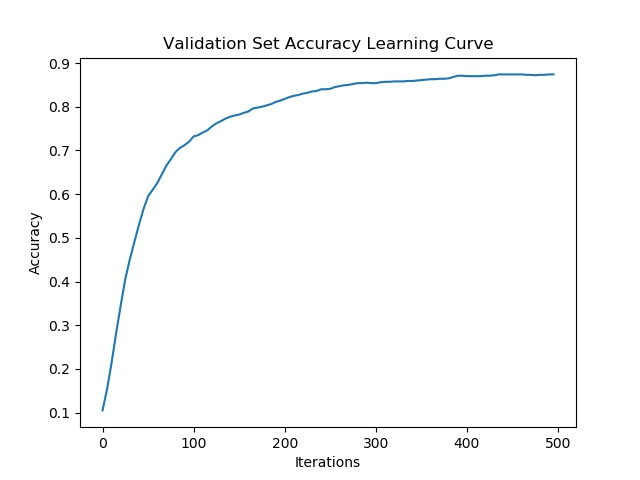
\includegraphics[width=\textwidth]{images/p4_valid_set_acc.jpeg}
    	\caption{Performance Curve on the Validation Set}
		\label{fig:part4validPerf}
	\end{subfigure}
%
	\begin{subfigure}[b]{0.5\textwidth}
		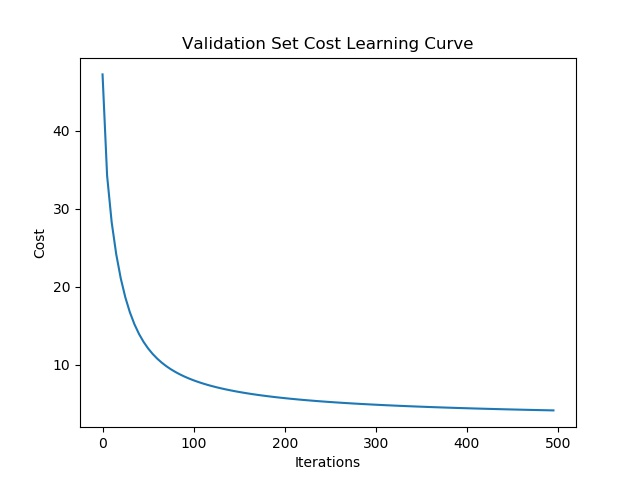
\includegraphics[width=\textwidth]{images/p4_valid_set_cost.jpeg}
		\caption{Loss Curve on the Validation Set}
		\label{fig:part4validLoss}
	\end{subfigure}
   \caption{Part 4 Learning Curves}
	\label{fig:part4curves}
\end{figure}
\newline
\newline
\noindent \textit{Weights Going Into Output Units}
\newline
Words
\clearpage
\end{homeworkProblem}


% Part 5
\begin{homeworkProblem}
	
	
	
	\begin{figure}[!ht]
	\begin{subfigure}[b]{0.5\textwidth}
    	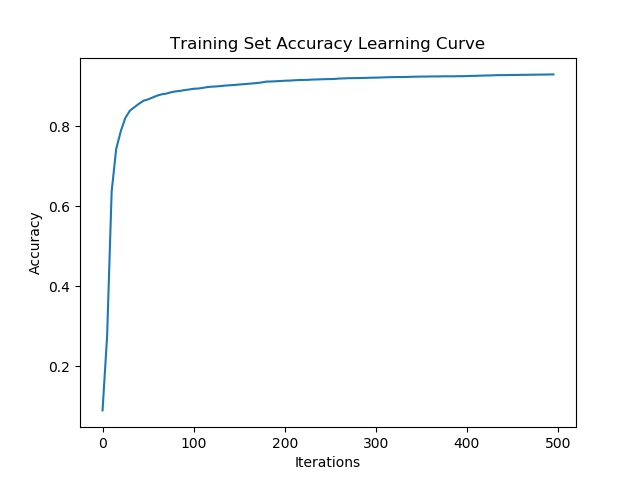
\includegraphics[width=\textwidth]{images/p5_training_set_acc.jpeg}
    	\caption{Performance Curve on the Training Set}
		\label{fig:part5trainPerf}
	\end{subfigure}
%
	\begin{subfigure}[b]{0.5\textwidth}
		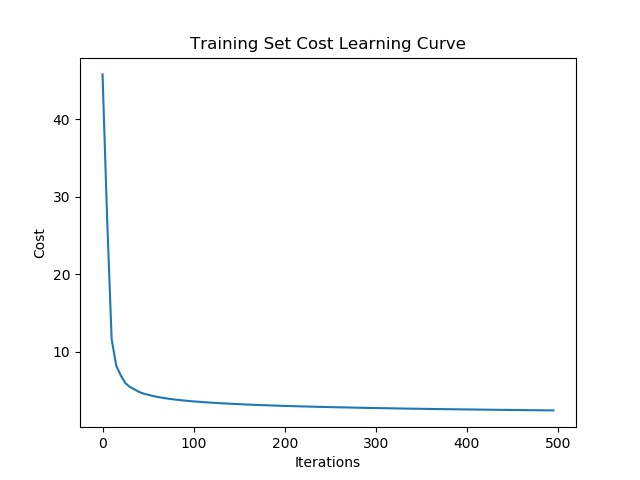
\includegraphics[width=\textwidth]{images/p5_training_set_cost.jpeg}
		\caption{Loss Curve on the Training Set}
		\label{fig:part5trainLoss}
	\end{subfigure}
    %	
	\begin{subfigure}[b]{0.5\textwidth}
    	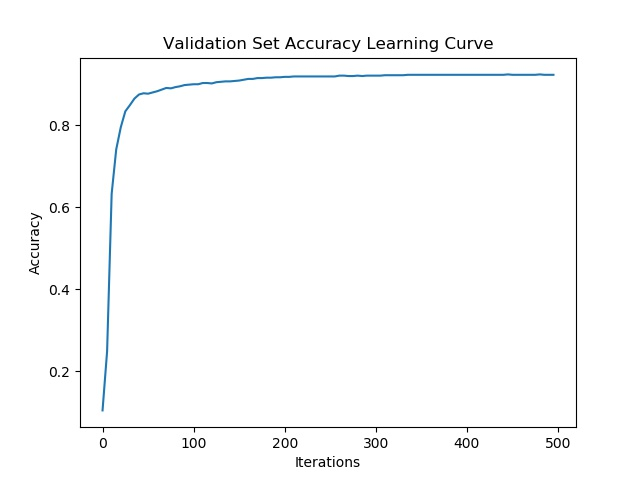
\includegraphics[width=\textwidth]{images/p5_valid_set_acc.jpeg}
    	\caption{Performance Curve on the Validation Set}
		\label{fig:part5validPerf}
	\end{subfigure}
%
	\begin{subfigure}[b]{0.5\textwidth}
		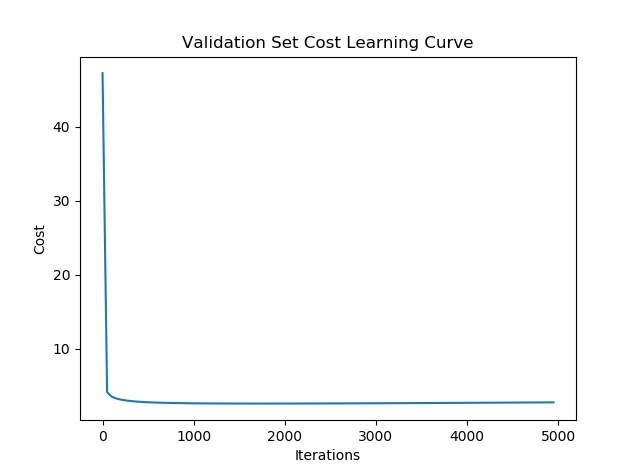
\includegraphics[width=\textwidth]{images/p5_valid_set_cost.jpeg}
		\caption{Loss Curve on the Validation Set}
		\label{fig:part5validLoss}
	\end{subfigure}
    \caption{Part 5 Learning Curves}
	\label{fig:part5curves}
\end{figure}

\clearpage

\begin{figure}[!ht]
	\begin{lstlisting}    
def part5_gradient_descent(X, Y, init_W, alpha, eps, max_iter, init_v, momentum):
	'''
	part5_gradient_descent finds a local minimum of the hyperplane defined by
	the hypothesis dot(W.T, X). The algorithm terminates when successive
	values of W differ by less than eps (convergence), or when the number of
	iterations exceeds max_iter. This function uses momentum
	
	Arguments:
		X -- input data for X (the data to be used to make predictions)
		Y -- input data for X (the actual/target data)
		init_W -- the initial guess for the local minimum (starting point)
		alpha -- the learning rate; proportional to the step size
		eps -- used to determine when the algorithm has converged on a solution
		max_iter -- the maximum number of times the algorithm will loop before
		terminating
		init_v -- the initial momentum value
		momentum -- the momentum parameter in range (0, 1)
	'''
	
	iter = 0
	previous_W = 0
	current_W = init_W.copy()
	previous_v = 0
	current_v = init_v # Initial momentum...
	firstPass = True
	history = list()
	Whistory = list()
	
	m = Y.shape[1]
	
	# Do-while...
	while(firstPass or
			(np.linalg.norm(current_W  - previous_W) > eps and 
			iter < max_iter)):
		firstPass = False
		
		previous_W = current_W.copy() # Update the previous W value
		previous_v = current_v # Update previous momentum
		
		current_v = momentum * current_v + alpha * p3.negLogLossGrad(X, Y, current_W)
		current_W = current_W - current_v
		
		if(iter % (max_iter // 100) == 0):
			# Print updates every so often and save cost into history list
			cost = p3.NLL(p2.SimpleNetwork(current_W, X), Y)
			history.append((iter, cost))
			Whistory.append(current_W)
			print("Iter: ", iter, " | Cost: ", cost)
		
		iter += 1
	
	return(Whistory, history)
	\end{lstlisting}
	\caption{Vectorized Code for Gradient Descent with Momentum}
	\label{fig:part5_code}
\end{figure}
\clearpage
\end{homeworkProblem}


% Part 6
\begin{homeworkProblem}
	\noindent \textit{Comparison Between Momentum and Vanilla Gradient Descent}
\newline
The effect of momentum on gradient descent was studied by taking two different weights, treating them as coordinates and plotting their path over 20 iterations on a contour plot. Gradient descent was run two times for each plot, using the same initial weight matrices and only changing the two chosen weights while keeping the other weights constant. The coordinates of the weights studied were $W[200, 2]$ and $W[201, 2]$. Figure~\ref{fig:part6Equal} shows a plot where the two methods were comparable.\newline
		
		\noindent \textit{Results}

It was found that the effects of momentum could be seen most clearly when the learning rate was slightly increased, shown in Figure~\ref{fig:part6Mom}. This is because in the vanilla method, the weights would travel mostly vertically, due to the shape of the contour, while in the momentum method, the vertical components of the weights would cancel each other out over consecutive steps.

However, when momentum is too high, the contributions from the previous steps would have too much of an effect, resulting in the weights overshooting the minimum like in Figure~\ref{fig:part6Van}.

\begin{figure}[!ht]

	\begin{subfigure}[b]{0.5\textwidth}
    	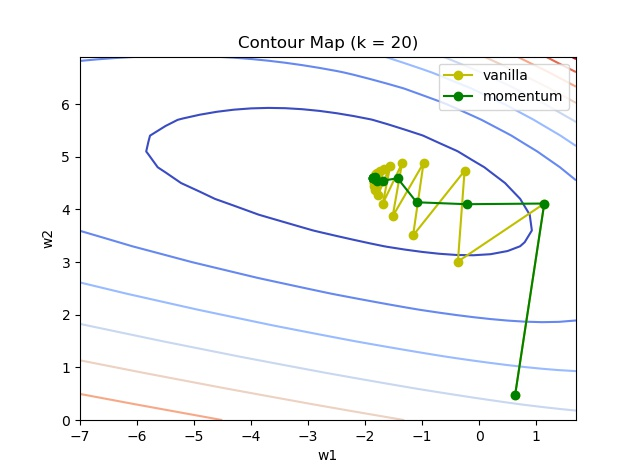
\includegraphics[width=\textwidth]{images/contour_20k_05a_03mom.jpeg}
    	\caption{Alpha = 0.5, Momentum = 0.3}
		\label{fig:part6Equal}
	\end{subfigure}
%
	\begin{subfigure}[b]{0.5\textwidth}
		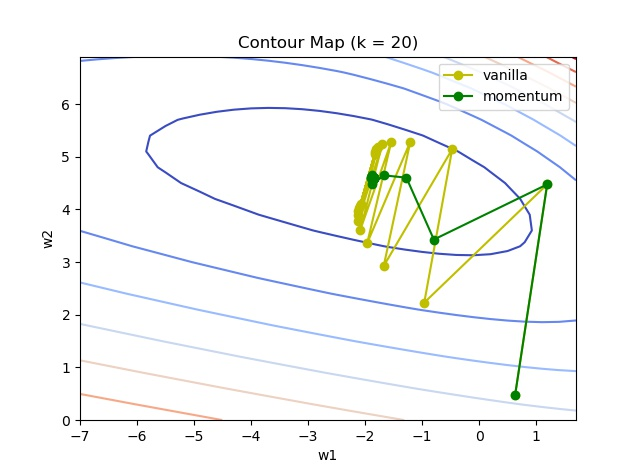
\includegraphics[width=\textwidth]{images/contour_20k_055a_03mom.jpeg}
		\caption{Alpha = 0.55, Momentum = 0.3}
		\label{fig:part6Mom}
	\end{subfigure}
    %	
	\begin{subfigure}[b]{0.5\textwidth}
		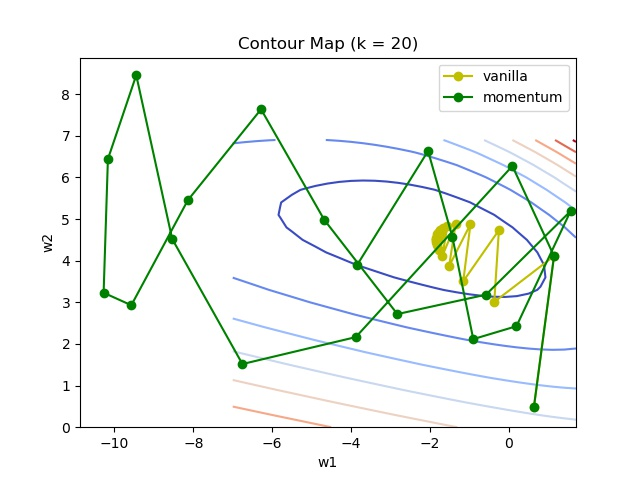
\includegraphics[width=\textwidth]{images/contour_20k_05a_09mom.jpeg}
		\caption{Alpha = 0.5, Momentum = 0.9}
	\label{fig:part6Van}
	\end{subfigure}
	\caption{Contour Plots}
	\label{fig:part6}
\end{figure}
\clearpage
\end{homeworkProblem}


% Part 7
\begin{homeworkProblem}
\noindent \textit{The Effect of Caching on the Time Required to Compute the Gradient}
\newline
A neural network consists of several layers of \textit{neurons} connected to each other by edges which each have their own \textit{weight}. In order to optimize a neural network, we need to ``learn" the values for the weights that minimize the cost function. The \textit{gradient} of the cost function can be computed with respect to each weight in the network; this matrix-valued quantity indicates (up to a proportionality constant) how much each of the weights should be changed to achieve the target output. Traditionally, there are two algorithms that come to mind for how to compute the gradient, both of which make excessive use of the chain rule from calculus:
\begin{enumerate}[(1)]
	\item Na\"ive approach: brute-force computation of the gradient, where each entry in the gradient matrix is evaluated separately.
	\item Better approach: ``backpropagation", a computation of the gradient that uses caching to store each partial derivative so that no term ever has to be computed twice. Terms are accessed from a table in $O(1)$ time once they have been computed, and are added to the table otherwise.
\end{enumerate}
This section presents an analysis of the runtime complexity of these two algorithms, ultimately deriving asymptotic upper bounds for each in the case of a fully-connected network with $N$ layers and $K$ neurons per layer. Note that only one training example will be considered, while in general the gradient would be an average over all training examples. The variables and dimensions to be used are explained as follows:
\begin{itemize}
	\item $C$ is the cost function
	\item $W^{(i, j, k)}$ is the weight corresponding to the edge connecting the $j$\textsuperscript{th} neuron in the $(i-1)$\textsuperscript{th} layer to the $i$\textsuperscript{th} neuron in the $i$\textsuperscript{th} layer
	\begin{itemize}
		\item $i \in [1, N]$
		\item $j, k \in [1, k]$
	\end{itemize}
	\item $a^{(i)} _k$ is the output from the $k$\textsuperscript{th} neuron in the $i$\textsuperscript{th} layer. Note that the neurons $a^{(0)} _k$ form the input layer and the neurons $a^{(N)} _k$ form the output layer.
	\item $N$ is the number of layers in the network
	\item $K$ is the number of neurons per layer
\end{itemize}
Also, the following reasonable assumptions are made to simplify the analysis:
\begin{enumerate}
	\item Element-wise multiplication is $O(1)$
	\item Addition is negligible
	\item Assume that an N-layer neural network includes the input and output layers in the count; that is, it has $N-2$ hidden layers
	\item Assume activations functions and non-linearities such as softmax at the output layer can be ignored
	\item Partial derivatives in tables (i.e. previously-solved subproblems) take negligible time to retrieve
\end{enumerate}
\noindent \textit{Characterization of Na\"ive Approach (Brute Force)}
\newline
We begin with the na\"ive approach as this will make the analysis for the ``better" approach more simple due to the terminology developed. We begin by writing the derivative of the cost function with respect to an arbitrary weight:

$$
\frac{\partial C}{\partial W^{(i, j, k)}}
$$

Next, we consider the fact that the cost function is evaluated at the output neurons, $a^{(N)} _ k$; that is, $C = C(a^{(N)} _1,...,a^{(N)} _K)$. Each $a^{(N)} _ k$ is in turn computed by first evaluating the inner product $\sum_{j = 1}^{K} W^{(N-1, j, k)}a^{(N-1)} _ j$, which uses the outputs from layer $N-1$ and the weights connecting these outputs to neuron $k$ in layer $N$. Each $a^{(N-1)} _ j$ can also be computed in a similar fashion using the outputs and weights from the previous layer, until layer $1$ is reached, which is the input layer. What this means is that any $a^{(i)} _k$ is technically an input to the cost function, so it makes sense to write expressions such as $\frac{\partial C}{\partial a^{(i)} _k}$. In fact, we can relate this to the partial derivative with respect to an arbitrary weight in the network using the chain rule from calculus:

$$
\frac{\partial C}{\partial W^{(i, j, k)}}
=
\frac{\partial C}{\partial a^{(i)} _k} % times
\frac{\partial a^{(i)} _k}{\partial W^{(i, j, k)}}
$$

But we can expand $\frac{\partial C}{\partial a^{(i)} _k}$ in terms of the $a_k$'s that are affected in the next layer by an infinitesimal change in $a^{(i)} _k$ (note that we sum from $1$ to $K$ because we are studying a fully-connected network and hence $a^{(i)} _k$ connects to $K$ neurons in the next layer):

$$
\frac{\partial C}{\partial a^{(i)} _k}
=
\sum_{l = 1}^{K}
	\Big(
		\frac{\partial C}{\partial a^{(i+1)} _l} % times
		\frac{\partial a^{(i+1)} _l}{\partial a^{(i)} _k}
	\Big)
$$

This expansion gives yet a larger expression for the derivative of the cost function with respect to an arbitrary weight:

$$
\frac{\partial C}{\partial W^{(i, j, k)}}
=
\frac{\partial C}{\partial a^{(i)} _k} % times
\frac{\partial a^{(i)} _k}{\partial W^{(i, j, k)}}
=
\bigg(
\sum_{l = 1}^{K}
\Big(
\frac{\partial C}{\partial a^{(i+1)} _l} % times
\frac{\partial a^{(i+1)} _l}{\partial a^{(i)} _k}
\Big)
\bigg)
\frac{\partial a^{(i)} _k}{\partial W^{(i, j, k)}}
=
\frac{\partial a^{(i)} _k}{\partial W^{(i, j, k)}}
\sum_{l = 1}^{K}
\Big(
\frac{\partial C}{\partial a^{(i+1)} _l} % times
\frac{\partial a^{(i+1)} _l}{\partial a^{(i)} _k}
\Big)
$$

Consider the case where we are interested in $\frac{\partial C}{\partial W^{(1, j, k)}}$, that is, the derivative of the cost function with respect to a weight connecting the input layer and layer $1$. In this case, the expansion has $N$ summation terms involving weights in the next layers:

$$
\frac{\partial C}{\partial W^{(1, j, k)}}
=
\frac{\partial a^{(1)} _k}{\partial W^{(1, j, k)}}
\sum_{l_1 = 1}^{K}
\Big( %1
	\frac{\partial a^{(2)} _{l_1}}{\partial a^{(1)} _k}
	\sum_{l_2 = 1}^{K}
	\Big(  %2
		\frac{\partial a^{(3)} _{l_2}}{\partial a^{(2)} _{l_1}}
		\sum_{l_3 = 1}^{K}
		\Big(  %3
			...\quad\quad...
			\sum_{l_{N-1} = 1}^{K}
			\Big(  %N-1
				\frac{\partial a^{(N-1)} _{l_{N-1}}}{\partial a^{(N-2)} _{l_{N-2}}}
				\sum_{l_N = 1}^{K}
				\Big(  %N
					\frac{\partial a^{(N)} _{l_N}}{\partial a^{(N-1)} _{l_{N-1}}}
				\Big) %N
			\Big) %N-1
		\Big) %3
	\Big) %2
\Big) %1
$$
Since there are $N$ sums, and each runs from $1$ to $K$, this computation of the gradient with respect to a weight between the input layer and the first layer involves $k^N$ operations, provided that the previously-stated assumptions hold. Thus, it follows that for a weight connecting the first and second layers, there are $k^{N-1}$ computations (since the indices in the previous expression would all begin at layer $2$ instead of layer $1$). Indeed, for the gradient with respect to any weight connecting neurons in the $(i-1)$\textsuperscript{th} and $i$\textsuperscript{th} layers, there are $k^{N-(i-1)}$ computations. Thus, for weights connecting the $N-1$\textsuperscript{th} and $N$\textsuperscript{th} layers, there are then $k^{N-(N-1)}=k$ computations.
\newline
\newline
The total number of operations is then:

$$
k(k^N + K^{N-1} + ... + k) = k^{N+1} + k^{N} + ... + k^2 \in O(Nk^{N+1})
$$

So the na\"ive algorithm has a runtime complexity that is asymptotically bounded above by $O(Nk^{N+1})$.
\clearpage

\noindent \textit{Characterization of Backpropagation}
\newline
Now we will analyse the ``better" solution, backpropagation. Intuitively, we expect that after computing each partial derivative once, we should never need to compute it again as this exemplifies an \textit{overlapping subproblem}. To illustrate this, note that the partial derivative of the cost function in the first layer (implicitly) uses the partial derivatives of the cost function with respect to the outputs and weights in the second layer, and so forth. These latter partial derivatives should be retrievable in constant time if they were computed earlier.
\newline
\newline
Note the following:
\begin{enumerate}
	\item Fully connected implies $k \times k = k^2$ weights per inter-layer junction
	\item $N$ layers implies $N-1$ inter-layer junctions
	\item Each partial derivative should be constant time to compute
	\item $(N-1)k^2$ total weights in the network
\end{enumerate}
Now, in the final layer of the network, there is $1$ partial derivative to compute for each $a^{(N)} _k$, which is simply $\frac{\partial C}{\partial a^{(N)} _k}$. However, in the previous inter-layer junction (i.e. connecting the $(N-1)$\textsuperscript{th} layer to the $N$\textsuperscript{th} layer), there are $2$ partial derivatives to compute, as shown below:

$$
\frac{\partial C}{\partial W^{(i, j, k)}}
=
\frac{\partial C}{\partial a^{(N)} _k} % times
\frac{\partial a^{(N)} _k}{\partial W^{(N, j, k)}}
$$

But ${\partial a^{(N)} _k}$ is computed when considering the derivative of the cost function with respect to the output layer. So, if we work backwards through the neural network, we can see we can save time on computation since we don't need to keep computing partial derivatives whose values we already know. That is, in the case shown above, there were two partial derivatives that needed to be computed, but only one of them would need to be computed if the derivatives in the previous layer were already solved.
\newline
\newline
This concept generalizes across the network; thus, since there is one new computation required per weight, and there are $k^2$ weights per inter-layer junction, the total number of computations required to solve the gradient of the network with respect to all weights is:

$$
k^2 + k^2 + ... + k^2 \quad\quad\quad\quad \text{$N$ times}
$$

This gives an asymptotic upper bound on the runtime complexity of $O(k^2 N)$.
\clearpage
\end{homeworkProblem}


% Part 8
\begin{homeworkProblem}
		\noindent \textit{Implementation of a Fully Connected Neural Network in PyTorch}
		
		A fully connected neural network was implemented in PyTorch with a single hidden layer and 6 output nodes. The network was trained on the faces of the 6 actors from project 1: Lorraine Bracco, Peri Gilpin, Angie Harmon, Alec Baldwin, Bill Hader and Steve Carell.\newline
		
		\noindent \textit{Image Processing}
		
		The number of photos used per actor for each set was 70 for the training set and 20 for both validation and test sets. To obtain each set, the uncropped photos from project1 were processed using the $make3Sets()$ function found in $image\_processing.py$, which creates the 3 sets of colored photos at the desired resolution. The function also compares the hashes of each photo to their expected hashes given by $actors.txt$ but some of the valid photos were wrongly skipped so they were hard coded back in. \newline
		
		\noindent \textit{Creation of Input Matrices}
		
		To create the input matrices for each set, each color channel of a photo was flattened into a 1D vector and concatenated along the 1D axis. This input vector was then stacked on to of a matrix which contained the input vectors of the other images in the set. In the resulting matrix, each row represented a different image while each column represented one of 3 colour values of a single pixel. The label matrices of each set were created by one hot encoding a 1 by 6 vector and stacking them on top of each other.\newline
		
		\noindent \textit{Final Results}
		
		The properties of the final and best performing network created can be seen in Table~\ref{tab:part8_properties}. The network's final performance on both validation and test sets was 82.5\% correct. The learning curves at these settings for both test and validation sets are shown in Figure~\ref{fig:part8curves}.
		
\begin{table}[!ht]
\begin{center}
\begin{tabular}{ | m{5.5cm} | m{12em}|}
\hline
\textbf{Property} & \textbf{Value} \\
\hline
Input Resolution & 28x28 \\ 
\hline
Input Layer Size & $28*28*3$\\ 
\hline
Hidden Layer Size & 70\\ 
\hline
Output Layer Size & 6\\ 
\hline
Hidden Layer Activation Function & Tanh\\ 
\hline
Loss Function & Cross Entropy Loss\\ 
\hline
Optimizer & Adam\\ 
\hline
Learning Rate & 1e-3\\ 
\hline
Batch Size & 60\\ 
\hline
Steps & 500\\ 
\hline
Initial Weights & Default Values\\ 
\hline
\end{tabular}
\end{center}
\caption{Properties of the Best Performing Neural Network}
\label{tab:part8_properties}
\end{table}

\begin{figure}[!ht]
	\begin{subfigure}[b]{0.5\textwidth}
    	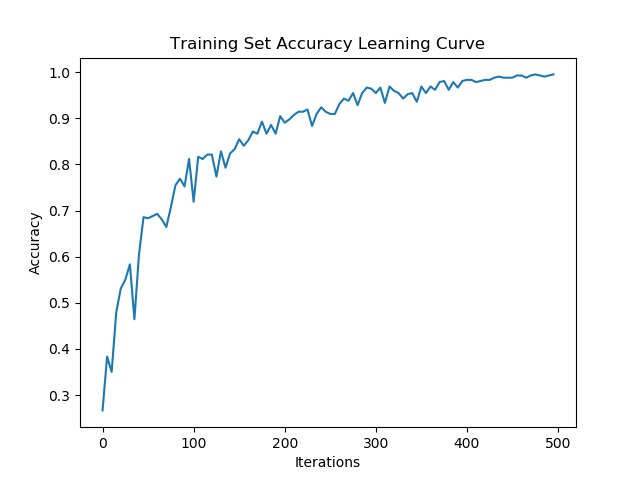
\includegraphics[width=\textwidth]{images/p8_training_set_acc.jpeg}
    	\caption{Performance Curve on the Training Set}
		\label{fig:part8trainPerf}
	\end{subfigure}
%
	\begin{subfigure}[b]{0.5\textwidth}
		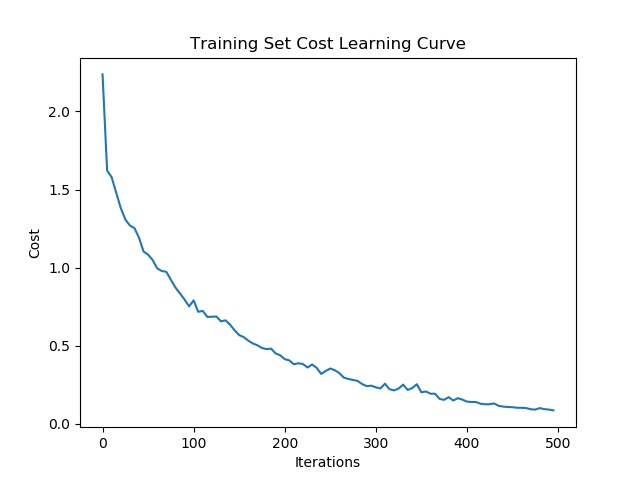
\includegraphics[width=\textwidth]{images/p8_training_set_cost.jpeg}
		\caption{Loss Curve on the Training Set}
		\label{fig:part8trainLoss}
	\end{subfigure}
    %	
	\begin{subfigure}[b]{0.5\textwidth}
    	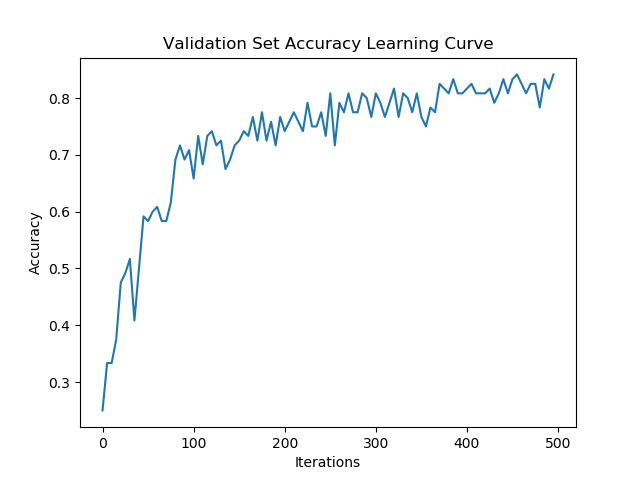
\includegraphics[width=\textwidth]{images/p8_valid_set_acc.jpeg}
    	\caption{Performance Curve on the Validation Set}
		\label{fig:part8validPerf}
	\end{subfigure}
%
	\begin{subfigure}[b]{0.5\textwidth}
		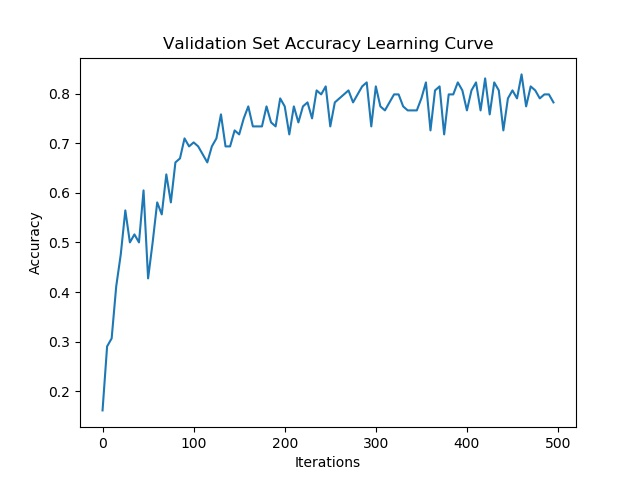
\includegraphics[width=\textwidth]{images/p8_valid_set_cost.jpeg}
		\caption{Loss Curve on the Validation Set}
		\label{fig:part8validLoss}
	\end{subfigure}
   \caption{Part 8Learning Curves}
	\label{fig:part8curves}
\end{figure}

\noindent \textit{Experimental Observations for Part 8}

\noindent \textit{The Effect of Resolution on Performance}

		The network was trained on square images at varying resolutions by making the input layer a function of the resolution. The resolutions used include: 64x64, 32x32, 28x28, 24x24 and 14x14. It was found that images close to 32x32 in size resulted in the best performance while those at resolutions of 14x14 and 64x64 gave slightly lower performances. It was also found that a larger resolution such as 64x64 required a much larger hidden layer to optimize than lower hidden layers.\newline
		
\noindent \textit{The Effect of Activation Functions on Performance}		
		
		Different activation functions for the hidden layer were also tested and it was found that as long as the hidden layer is large enough, (ie. ~50 nodes), most activation functions only made a few percentage difference. However, certain activation functions such as Softmin and Softmax would perform poorly no matter the size of the hidden layer.
		When the hidden layer was small,(ie. ~6 nodes), it was found that the best activation functions were relatively linear functions that could take both positive and negative values such as linear, Tanhshrink and Softshrink.\newline
		
		\noindent \textit{Weight Initialization}
		
	Different methods were tried to initialize the weights using functions such as normal\_(), uniform\_() and zero() with various parameters. It was found that if the weights are too large then the performance stays constant at 1/6. The weights that gave the best performance were the default weights.\newline
	
		Different loss functions and optimizers were also attempted but it was found that most loss functions required a different format of input so it was kept as $CrossEntropyLoss()$ while Adam was confirmed to be the best optimizer. 
\clearpage
\end{homeworkProblem}


% Part 9
\begin{homeworkProblem}
\noindent \textit{Visualizing the Weights of ``Useful" Hidden Units}

	The single-hidden-layer fully-connected network presented in part 8 was explored in greater depth in this part of the project. Consider the task of classifying images of just one actor, for example, Angie Harmon. Since the label vector, $y$, used a one-hot encoding scheme, a ``perfect" classification of an image of Harmon would have resulted in the output $[0\quad0\quad1\quad0\quad0\quad0]^T$ from the neural network. Note that only one output neuron is activated; let this output neuron corresponding to the actor be called $o_i$. One can then inquire about which hidden units were the most important, or ``useful" in computing this classification correctly. This part of the project explored a way of determining which hidden units were the most ``useful" for classifying input photos of Angie Harmon and Peri Gilpin, and visualizing the weights going into these ``useful" hidden units from the input layer. \newline

\noindent \textit{Defining ``Useful"}

	It was assumed that there were $2$ ``useful" hidden units for each actor:
	
	\begin{enumerate}[(1)]
		\item The hidden unit with the \textit{maximum} input value to $o_i$. This hidden unit promotes the activation of $o_i$ the most.
		\item The hidden unit with the \textit{minimum} input value to $o_i$. This hidden unit inhibits the activation of $o_i$ the most.
	\end{enumerate}
	
	Note that \textit{input value} refers neither to the activation value of the hidden neuron nor the weight of the edge connecting the hidden neuron to $o_i$; rather, it refers to the product of these two quantities. This product represents the \textit{actual} contribution from the hidden unit. \newline

\noindent \textit{Procedure to Determine the Most ``Useful" Hidden Units}

	\begin{enumerate}[(1)]
		\item Pick the actor whose ``useful" hidden units are to be determined. This specifies an output neuron $o_i$ whose connections to the hidden layer will be studied
		
		\begin{enumerate}[(a)]
			\item Feed an input of the actor from the validation set into the neural network
			\item Observe the weights connecting the hidden layer to $o_i$
			\item Observe the activation values from the neurons in the hidden layer
			\item For each neuron in the hidden layer, multiply its activation value by the weight connecting it to $o_i$. This product represents the actual contribution from the hidden unit
			\item Record the indices for the ``useful" hidden units (as per the definition of ``useful" above
		\end{enumerate}
	
		\item Repeat the previous step for all images of the actor
		\item Pick the most frequently-occurring promoter neuron, and the most frequently-occurring inhibitor neuron. Continue to the next step, considering just these two neurons to be ``useful"
		\item Visualize the weights connecting the ``useful" hidden units to the input layer
		\item Repeat for the next actor
	\end{enumerate}

\clearpage
\noindent \textit{Comments on Weight Visualization}

	The weights connecting the hidden layer to the most ``useful" hidden units are presented below, with the weights for Angie Harmon in Figure~\ref{fig:part9imagesHarmon}, and the weights for Peri Gilpin in Figure~\ref{fig:part9imagesGilpin}. Since it is possible for weights to be both positive and negative, the positive and negative parts of the weights were plotted as two separate images; below, the positive parts of the weights are on the left while the negative parts are on the right. The omitted values were set to $0$ for each plot.To obtain the weight visualizations from the weight vectors, the portions of the weight vectors representing the red, green, and blue channels of the input images were reshaped back to a $2$-D color image.


\begin{figure}[!ht]
	\centering
	\begin{subfigure}[b]{1\textwidth}
		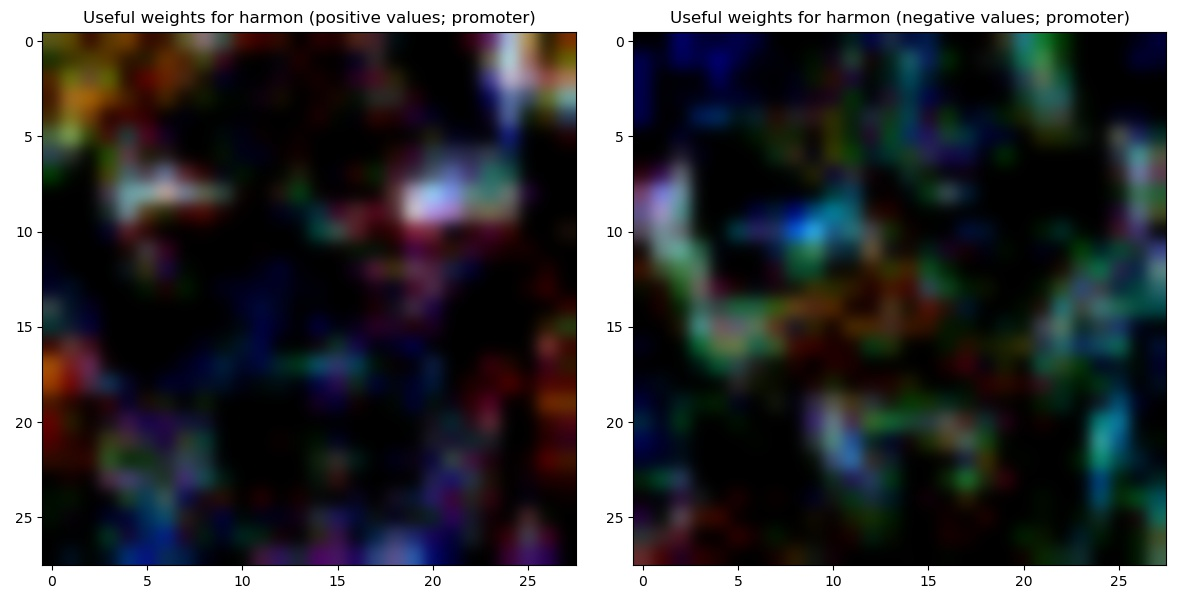
\includegraphics[width=\textwidth]{images/part8harmonpromoter}
		\caption{The hidden unit promoting the activation of Harmon the most.}
		\label{fig:part9HarmonPromoter}
	\end{subfigure}
	%
	\begin{subfigure}[b]{1\textwidth}
		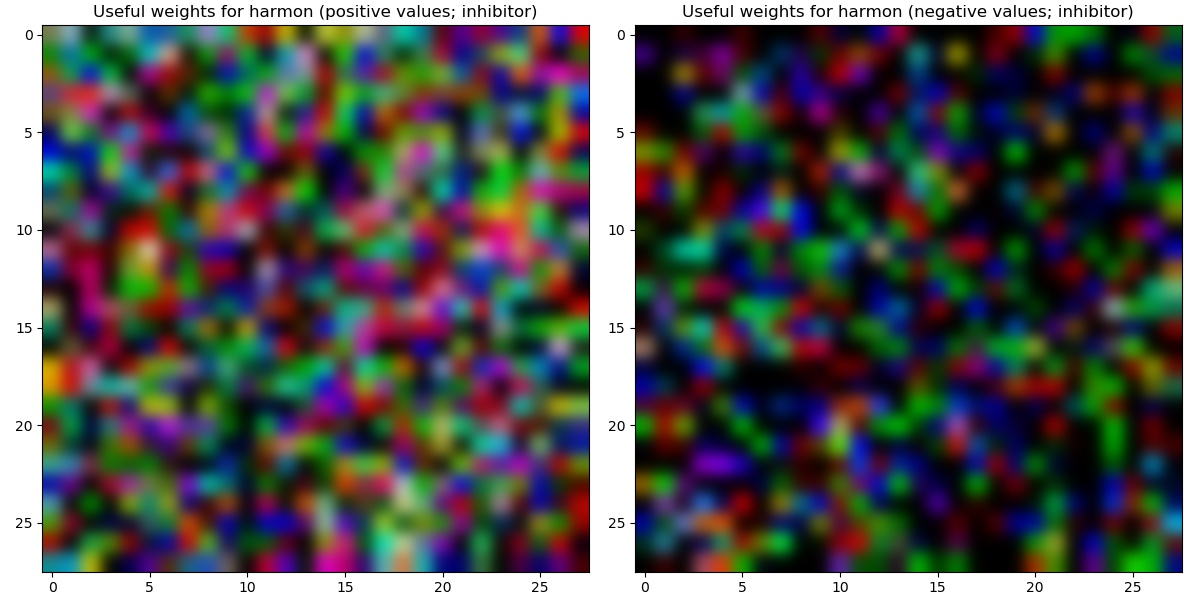
\includegraphics[width=\textwidth]{images/part8harmoninhibitor}
		\caption{The hidden unit inhibiting the activation of Harmon the most.}
		\label{fig:part9HarmonInhibitor}
	\end{subfigure}
	\caption{Weight visualizations for Angie Harmon.}
	\label{fig:part9imagesHarmon}
\end{figure}

\clearpage

\begin{figure}[!ht]
	\centering
	\begin{subfigure}[b]{1\textwidth}
		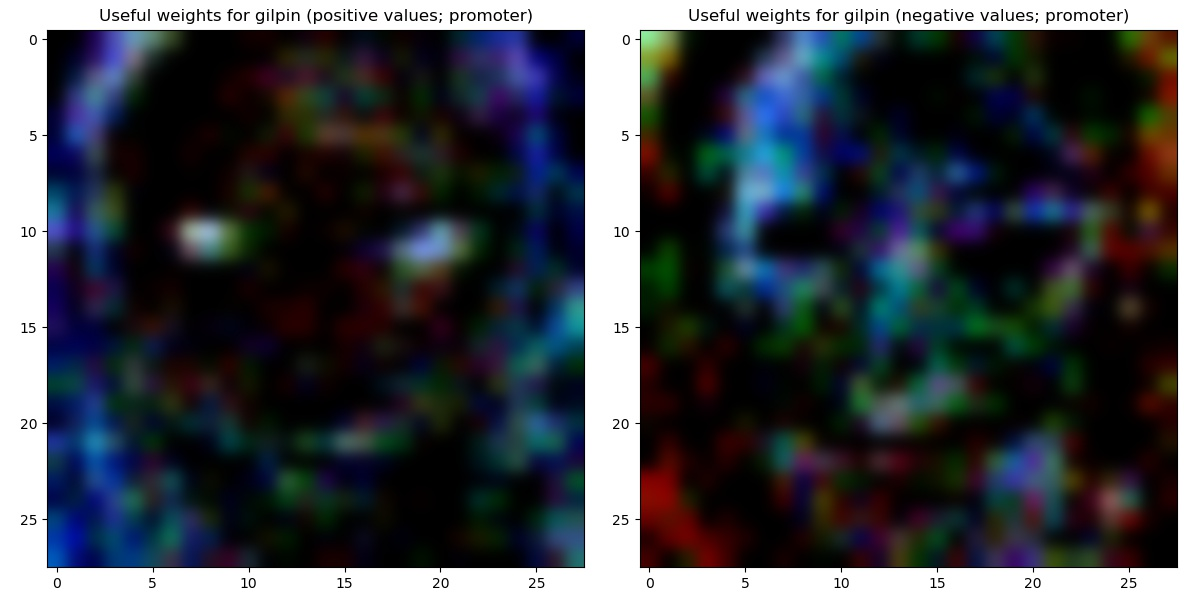
\includegraphics[width=\textwidth]{images/part8gilpinpromoter}
		\caption{The hidden unit promoting the activation of Gilpin the most.}
		\label{fig:part9GilpinPromoter}
	\end{subfigure}
	%
	\begin{subfigure}[b]{1\textwidth}
		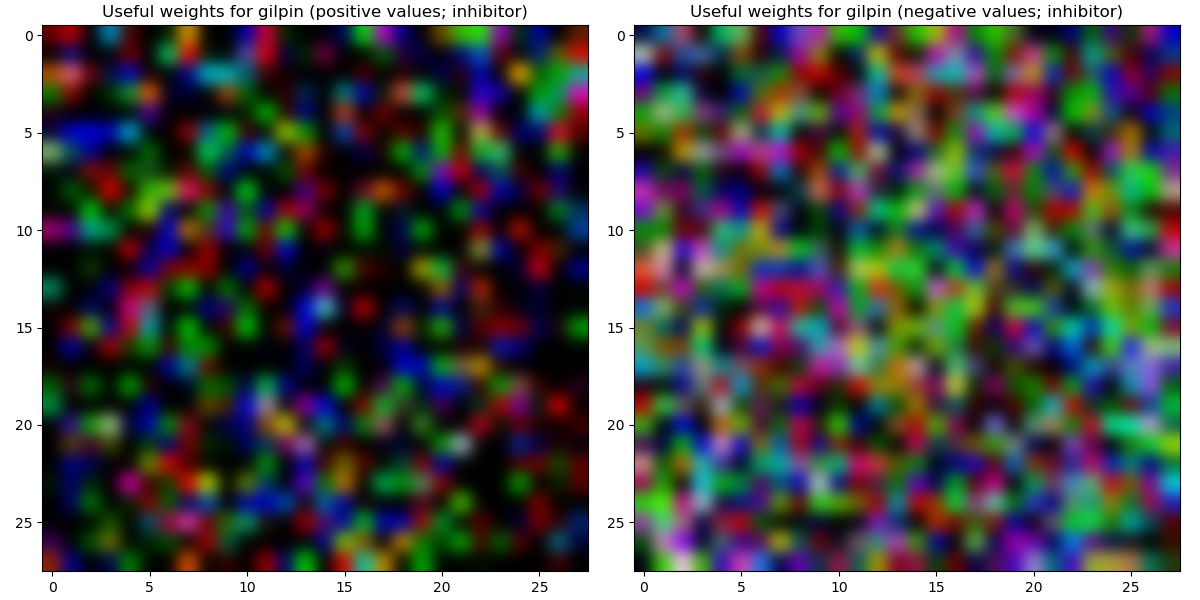
\includegraphics[width=\textwidth]{images/part8gilpininhibitor}
		\caption{The hidden unit inhibiting the activation of Gilpin the most.}
		\label{fig:part9GilpinInhibitor}
	\end{subfigure}
	\caption{Weight visualizations for Peri Gilpin.}
	\label{fig:part9imagesGilpin}
\end{figure}

\clearpage
\end{homeworkProblem}


% Part 10
\begin{homeworkProblem}
	\noindent \textit{Implementing a Fully Connected Neural Network on Top of MyAlexNet}	
	
	To increase the accuracy of classification, the images were put into MyAlexNet and outputs from its features layers were taken and connected to a fully connected network with 1 hidden layer. \newline
	
	\noindent \textit{Modifying MyAlexNet}	
	
	To access the Top feature layer of MyAlexNet, the classifier in the forward function was commented out and the output was reshaped into a 1D vector. To access deeper layers, they are commented out in the $self.features$ section of the class. For every convolutional layer that's commented out, we also comment out an in dex in the $features\_weight\_i$ array to prevent the program from trying to load weights into a non-existent layer.\newline
	
	\noindent \textit{Computing the Input Matrix for the Fully Connected Layers}	
	
	After MyAlexNet is modified to provide the desired output, we take each image in a set and put it into MyAlexNet using the sample code given, obtain its corresponding 1D vector and compile it into a set matrix. In the resulting matrix, each row represents an image in that set while each column represents an output of MyAlexNet corresponding to that image. The label matrices are created in the same way as in part 8.
		
	Since only the fully connected layers are trained, the training set matrix from MyAlexNet will always stay the same. Therefore, we can use the output of MyAlexNet as the new inputs to the the fully connected layers without having to recalculate them every time. The input layer of the fully connected layers also has to be resized to match the number of outputs from MyAlexNet.\newline
	
	\noindent \textit{Final Results}	
	
	The properties of the optimal configuration are shown in Table~\ref{tab:part10_properties}. The outputs from conv4 after the MaxPool layer and from conv2 after the ReLU layer were found to provide the best results but the latter, while having more outputs, gave slightly better performance. The final performance on the validation set was 96.6\% while the final performance on the test set was 98.33\%. This represents approximately a 70\% drop in the error rate from part 8. The learning curves of the test and validation sets are disaplayed in Figure~\ref{fig:part10curves}\newline
	
	\begin{table}[!ht]
\begin{center}
\begin{tabular}{ | m{5.5cm} | m{12em}|}
\hline
\textbf{Property} & \textbf{Value} \\
\hline
Input Resolution & 227x227 \\ 
\hline
MyAlexNet Output Layer & conv2 after ReLU \\ 
\hline
Input Layer Size & 64896\\ 
\hline
Hidden Layer Size & 50\\ 
\hline
Output Layer Size & 6\\ 
\hline
Hidden Layer Activation Function & Tanh\\ 
\hline
Loss Function & Cross Entropy Loss\\ 
\hline
Optimizer & Adam\\ 
\hline
Learning Rate & 1e-3\\ 
\hline
Batch Size & 50\\ 
\hline
Steps & 200\\ 
\hline
Initial Weights & Default Values\\ 
\hline
\end{tabular}
\end{center}
\caption{Properties of the Best Performing Neural Network}
\label{tab:part10_properties}
\end{table}

\begin{figure}[!ht]
	\begin{subfigure}[b]{0.5\textwidth}
    	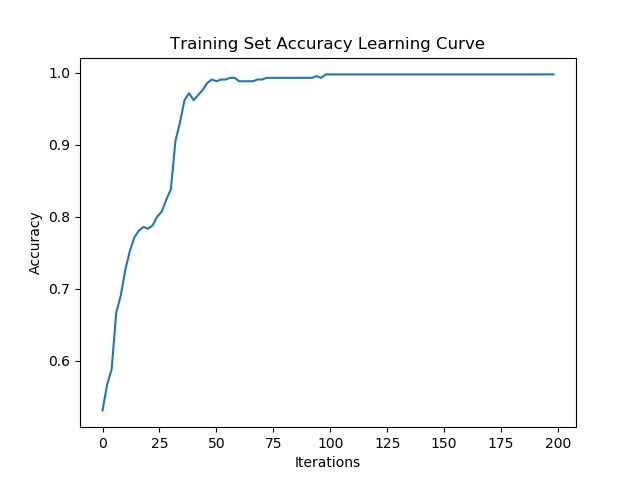
\includegraphics[width=\textwidth]{images/p10_training_set_acc.jpeg}
    	\caption{Performance Curve on the Training Set}
		\label{fig:part10trainPerf}
	\end{subfigure}
%
	\begin{subfigure}[b]{0.5\textwidth}
		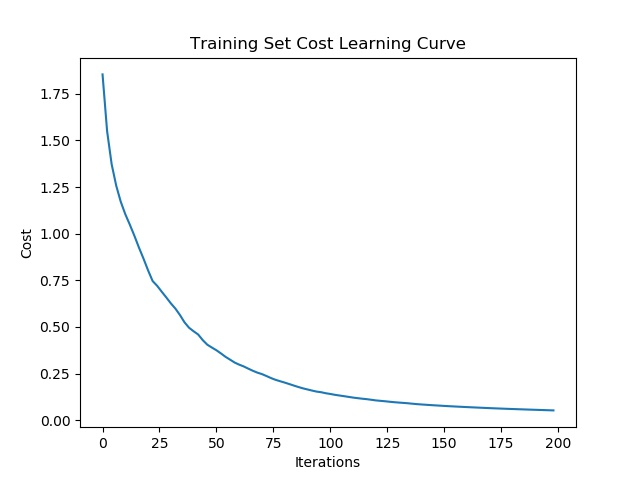
\includegraphics[width=\textwidth]{images/p10_training_set_cost.jpeg}
		\caption{Loss Curve on the Training Set}
		\label{fig:part10trainLoss}
	\end{subfigure}
    %	
	\begin{subfigure}[b]{0.5\textwidth}
    	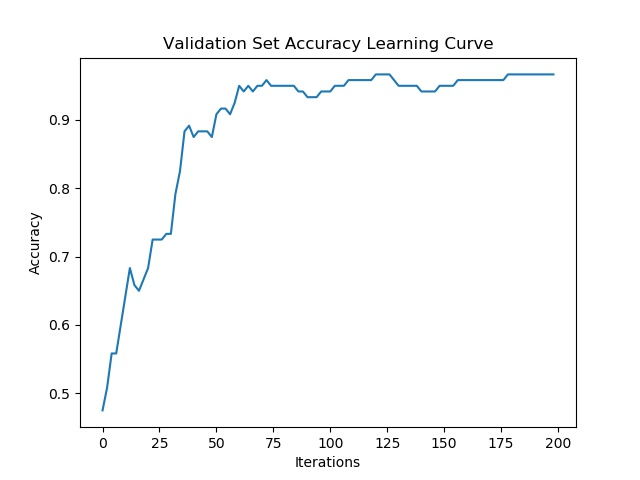
\includegraphics[width=\textwidth]{images/p10_valid_set_acc.jpeg}
    	\caption{Performance Curve on the Validation Set}
		\label{fig:part10validPerf}
	\end{subfigure}
%
	\begin{subfigure}[b]{0.5\textwidth}
		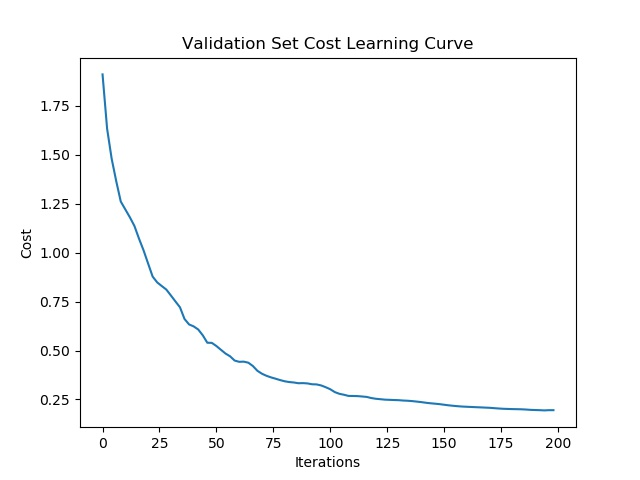
\includegraphics[width=\textwidth]{images/p10_valid_set_cost.jpeg}
		\caption{Loss Curve on the Validation Set}
		\label{fig:part10validLoss}
	\end{subfigure}
   \caption{Part 10 Learning Curves}
	\label{fig:part10curves}
\end{figure}
\clearpage
\end{homeworkProblem}


%----------------------------------------------------------------------------------------

\end{document}